% Unificación de arquitecturas como MPNNs
% Compilar con: pdflatex mpnn_unification.tex
\documentclass[tikz,border=10pt]{standalone}
\usepackage{tikz}
\usepackage{amsmath,amssymb}
\usepackage{xcolor}
\definecolor{gdlblue}{RGB}{41, 98, 168}
\definecolor{gdlred}{RGB}{191, 49, 49}
\definecolor{gdlgreen}{RGB}{30, 130, 76}
\definecolor{gdlorange}{RGB}{217, 130, 30}
\definecolor{gdlpurple}{RGB}{118, 56, 138}
\definecolor{gdlgray}{RGB}{140, 140, 140}
\definecolor{gdlyellow}{RGB}{190, 140, 10}
\usetikzlibrary{arrows.meta, positioning, calc, fit, backgrounds}

\begin{document}
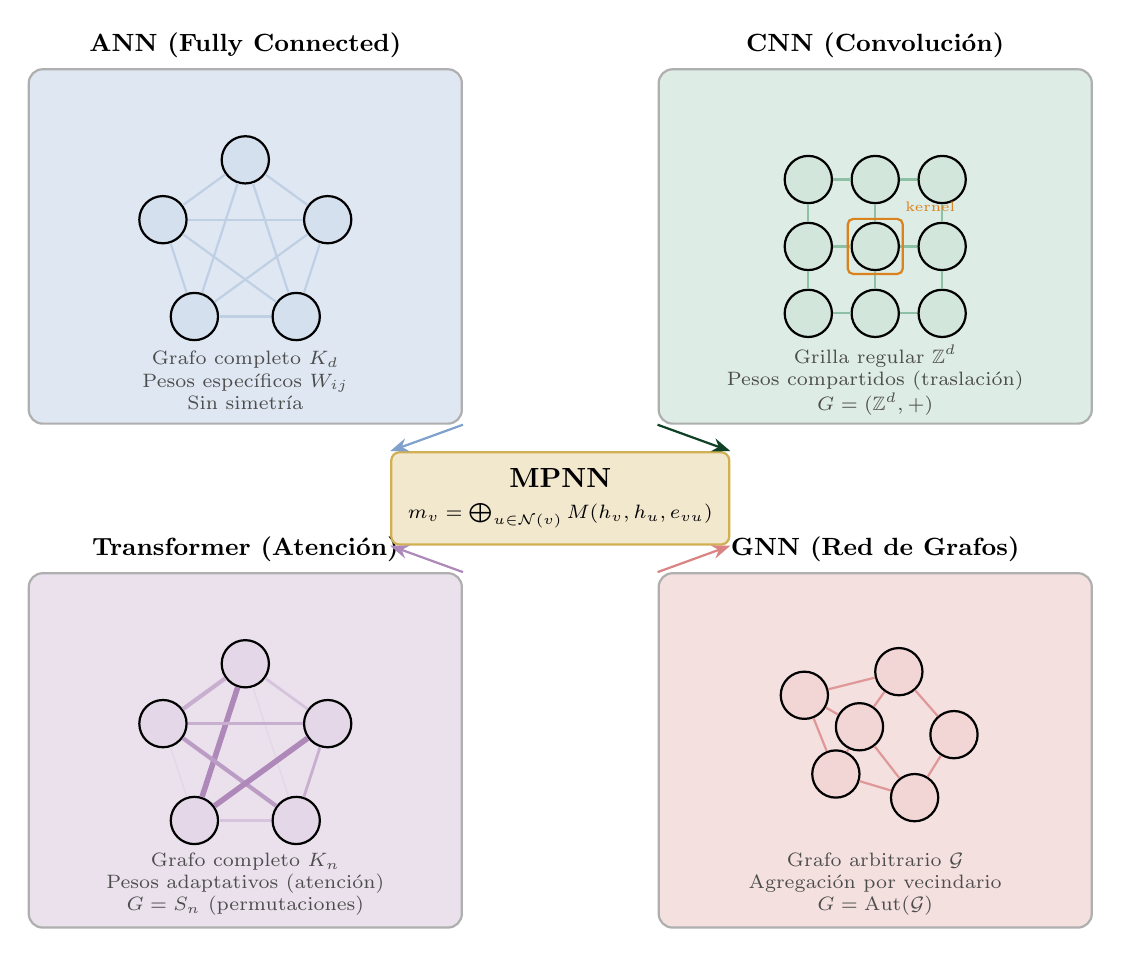
\begin{tikzpicture}[>=Stealth, font=\small,
    node/.style={circle, draw, thick, fill=white, minimum size=6mm, inner sep=0pt},
    edge/.style={thick, draw=gdlgray!60},
    box/.style={rectangle, rounded corners=5pt, draw=gdlgray!70, thick, minimum width=5.5cm, minimum height=4.5cm},
    title/.style={font=\small\bfseries, fill=white, inner sep=2pt},
    info/.style={font=\scriptsize, text=black!70, align=center}
]

% === ANN: Grafo completo, pesos específicos ===
\begin{scope}[shift={(-4, 3.2)}]
    \node[box, fill=gdlblue!15] (annbox) at (0, 0) {};
    \node[title] at (0, 2.55) {ANN (Fully Connected)};

    \foreach \i/\a in {1/90, 2/162, 3/234, 4/306, 5/18} {
        \node[node, fill=gdlblue!20] (a\i) at (\a:1.1) {};
    }
    % Todas las conexiones (grafo completo)
    \foreach \i in {1,...,5} {
        \foreach \j in {1,...,5} {
            \ifnum\i<\j
                \draw[edge, gdlblue!30] (a\i) -- (a\j);
            \fi
        }
    }

    \node[info] at (0, -1.7) {Grafo completo $K_d$\\Pesos específicos $W_{ij}$\\Sin simetría};
\end{scope}

% === CNN: Grilla regular, pesos compartidos ===
\begin{scope}[shift={(4, 3.2)}]
    \node[box, fill=gdlgreen!15] (cnnbox) at (0, 0) {};
    \node[title] at (0, 2.55) {CNN (Convolución)};

    % Grilla 3x3
    \foreach \i in {0,1,2} {
        \foreach \j in {0,1,2} {
            \node[node, fill=gdlgreen!20] (c\i\j) at ({\i*0.85 - 0.85}, {\j*0.85 - 0.85}) {};
        }
    }
    % Conexiones de grilla (horizontal y vertical)
    \foreach \i in {0,1,2} {
        \foreach \j [evaluate=\j as \jn using int(\j+1)] in {0,1} {
            \draw[edge, gdlgreen!50] (c\i\j) -- (c\i\jn);
            \draw[edge, gdlgreen!50] (c\j\i) -- (c\jn\i);
        }
    }
    % Resaltar kernel en nodo central
    \draw[thick, gdlorange, rounded corners=2pt] (-0.35, -0.35) rectangle (0.35, 0.35);
    \node[font=\tiny, gdlorange] at (0.7, 0.5) {kernel};

    \node[info] at (0, -1.7) {Grilla regular $\mathbb{Z}^d$\\Pesos compartidos (traslación)\\$G = (\mathbb{Z}^d, +)$};
\end{scope}

% === Transformer: Grafo completo, pesos adaptativos ===
\begin{scope}[shift={(-4, -3.2)}]
    \node[box, fill=gdlpurple!15] (transbox) at (0, 0) {};
    \node[title] at (0, 2.55) {Transformer (Atención)};

    \foreach \i/\a in {1/90, 2/162, 3/234, 4/306, 5/18} {
        \node[node, fill=gdlpurple!20] (t\i) at (\a:1.1) {};
    }
    % Conexiones con grosor variable (atención)
    \draw[edge, gdlpurple!60, line width=2pt] (t1) -- (t3);
    \draw[edge, gdlpurple!40, line width=1.5pt] (t1) -- (t2);
    \draw[edge, gdlpurple!20, line width=0.5pt] (t1) -- (t4);
    \draw[edge, gdlpurple!30, line width=1pt] (t1) -- (t5);
    \draw[edge, gdlpurple!50, line width=1.5pt] (t2) -- (t4);
    \draw[edge, gdlpurple!20, line width=0.5pt] (t2) -- (t3);
    \draw[edge, gdlpurple!40, line width=1pt] (t2) -- (t5);
    \draw[edge, gdlpurple!60, line width=2pt] (t3) -- (t5);
    \draw[edge, gdlpurple!30, line width=0.8pt] (t3) -- (t4);
    \draw[edge, gdlpurple!40, line width=1pt] (t4) -- (t5);

    \node[info] at (0, -1.7) {Grafo completo $K_n$\\Pesos adaptativos (atención)\\$G = S_n$ (permutaciones)};
\end{scope}

% === GNN: Grafo arbitrario ===
\begin{scope}[shift={(4, -3.2)}]
    \node[box, fill=gdlred!15] (gnnbox) at (0, 0) {};
    \node[title] at (0, 2.55) {GNN (Red de Grafos)};

    % Grafo irregular
    \node[node, fill=gdlred!20] (g1) at (-0.9, 0.7) {};
    \node[node, fill=gdlred!20] (g2) at (0.3, 1) {};
    \node[node, fill=gdlred!20] (g3) at (1, 0.2) {};
    \node[node, fill=gdlred!20] (g4) at (-0.5, -0.3) {};
    \node[node, fill=gdlred!20] (g5) at (0.5, -0.6) {};
    \node[node, fill=gdlred!20] (g6) at (-0.2, 0.3) {};

    \draw[edge, gdlred!50] (g1) -- (g2);
    \draw[edge, gdlred!50] (g1) -- (g4);
    \draw[edge, gdlred!50] (g1) -- (g6);
    \draw[edge, gdlred!50] (g2) -- (g3);
    \draw[edge, gdlred!50] (g2) -- (g6);
    \draw[edge, gdlred!50] (g3) -- (g5);
    \draw[edge, gdlred!50] (g4) -- (g5);
    \draw[edge, gdlred!50] (g4) -- (g6);
    \draw[edge, gdlred!50] (g5) -- (g6);

    \node[info] at (0, -1.7) {Grafo arbitrario $\mathcal{G}$\\Agregación por vecindario\\$G = \mathrm{Aut}(\mathcal{G})$};
\end{scope}

% === Flechas centrales hacia el marco MPNN ===
\node[font=\bfseries, align=center, fill=gdlyellow!20, rounded corners=3pt, draw=gdlyellow!70, thick, inner sep=6pt] (mpnn) at (0, 0) {MPNN\\[-1pt]{\scriptsize $m_v = \bigoplus_{u \in \mathcal{N}(v)} M(h_v, h_u, e_{vu})$}};

\draw[->, thick, gdlblue!60] (annbox.south east) -- (mpnn.north west);
\draw[->, thick, gdlgreen!50!black] (cnnbox.south west) -- (mpnn.north east);
\draw[->, thick, gdlpurple!60] (transbox.north east) -- (mpnn.south west);
\draw[->, thick, gdlred!60] (gnnbox.north west) -- (mpnn.south east);

\end{tikzpicture}
\end{document}
